\documentclass[border=6pt]{standalone}
\usepackage[T1]{fontenc}
\usepackage{lmodern}
\usepackage{tikz}
\usetikzlibrary{arrows.meta,positioning,shapes.geometric,calc,fit}
\begin{document}
\hyphenpenalty=10000 \exhyphenpenalty=10000
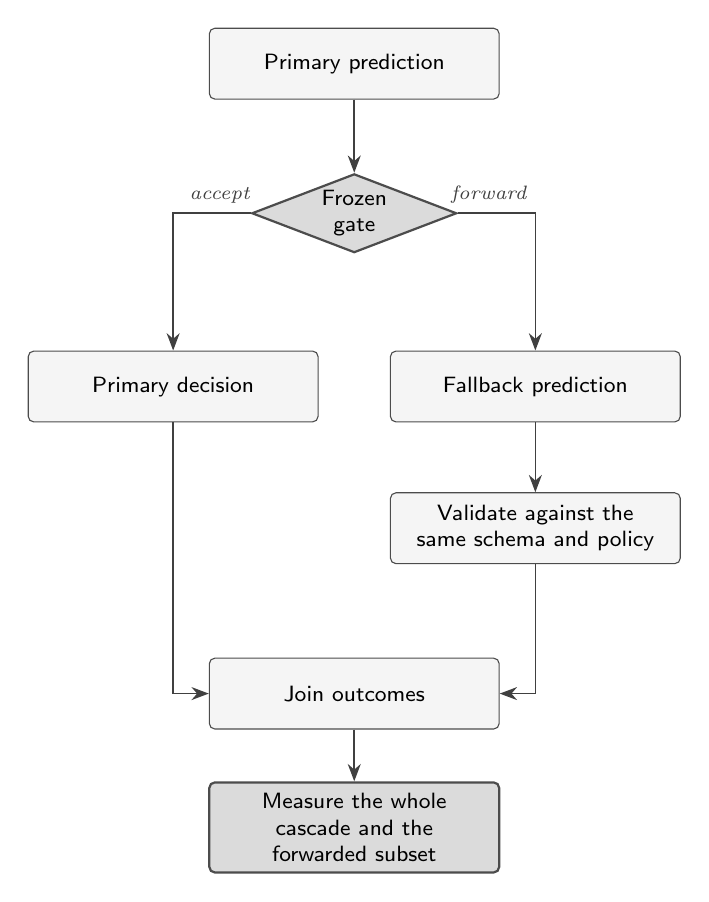
\begin{tikzpicture}[
  font=\footnotesize\sffamily,
  box/.style={draw=black!70, rounded corners=2pt, fill=black!4, align=center,
              text width=3.4cm, minimum height=0.9cm, inner sep=4pt},
  key/.style={box, fill=black!14, line width=0.8pt},
  dec/.style={diamond, aspect=2.6, draw=black!70, fill=black!14, align=center, inner sep=1pt, line width=0.8pt},
  arr/.style={-{Stealth[length=2.2mm]}, draw=black!75, line width=0.6pt},
  lab/.style={font=\scriptsize\itshape, text=black!75}
]
\node[box] (a) at (0,0) {Primary prediction};
\node[dec] (g) at (0,-1.9) {Frozen\\gate};
\node[box] (pd) at (-2.3,-4.1) {Primary decision};
\node[box] (fb) at (2.3,-4.1) {Fallback prediction};
\node[box] (vv) at (2.3,-5.9) {Validate against the same schema and policy};
\node[box] (j) at (0,-8.0) {Join outcomes};
\node[key] (ms) at (0,-9.7) {Measure the whole cascade and the forwarded subset};

\draw[arr] (a) -- (g);
\draw[arr] (g.west) -| (pd.north) node[lab, above, pos=0.2] {accept};
\draw[arr] (g.east) -| (fb.north) node[lab, above, pos=0.2] {forward};
\draw[arr] (fb) -- (vv);
\draw[arr] (pd.south) |- (j.west);
\draw[arr] (vv.south) |- (j.east);
\draw[arr] (j) -- (ms);
\end{tikzpicture}
\end{document}
